% =============================================================================
% Supporting Information for
% Declined, displaced, or just harder to catch? A simulation framework for
% attributing marine heatwave impacts on fished populations from catch per unit effort
% TEMPLATE: %%TAB:<name>%% lines are filled by scripts/assemble_manuscript.R,
% which writes manuscript/sim-rec_supp.tex.
% =============================================================================
\documentclass[11pt,a4paper]{article}
\usepackage[T1]{fontenc}
\usepackage{lmodern}
\usepackage[margin=25mm]{geometry}
\usepackage{amsmath,amssymb}
\usepackage{graphicx}
\graphicspath{{figures/}{../figures/}}
\usepackage{booktabs,array}
\usepackage[round]{natbib}
\usepackage{setspace}
\onehalfspacing
\usepackage{caption}
\captionsetup{font=small,labelfont=bf,labelsep=period,justification=raggedright,singlelinecheck=false}
\usepackage[hidelinks]{hyperref}
\usepackage{xurl}
\setlength{\emergencystretch}{2em}
\newcommand{\vt}[1]{\text{#1}}
\renewcommand{\thesection}{S\arabic{section}}
\renewcommand{\thetable}{S\arabic{table}}
\renewcommand{\thefigure}{S\arabic{figure}}
\renewcommand{\theequation}{S\arabic{equation}}

\title{Supporting Information for\\ \large Declined, displaced, or just harder to catch? A simulation framework for attributing marine heatwave impacts on fished populations from catch per unit effort}
\author{}
\date{}

\begin{document}
\maketitle

\noindent This document contains five supporting sections, nine tables and four figures referred to in the main text. Section, table and figure numbers in the main text refer to the main text; those prefixed S refer to this document.

% =============================================================================
\section{Why a fishery-independent survey is not simply another catch rate}
\label{sec:why-survey}

A survey also records catch and effort, so it is fair to ask how a survey index differs from the CPUE whose failure the main text establishes. The arithmetic is the same: both divide catch by effort. What differs is how the effort is placed and whether catchability is fixed, and those two properties, not the ratio itself, decide whether an index tracks abundance.

\paragraph{Where effort goes.} Commercial effort follows the fish. In the model the allocation weights depend on last month's catch rates, on distance from port and, during events, on the contraction term, so the spatial distribution of effort is correlated with the very state being estimated. Survey stations are drawn with known, equal inclusion probabilities that do not depend on abundance, which is what makes design-based inference possible \citep{sarndal1992}. The commercial index averages over a footprint the fleet selects; the survey index is a probability-weighted average over a footprint fixed in advance, which is why it is computed as a Horvitz--Thompson total \citep{horvitz1952} rather than as a raw ratio.

\paragraph{Whether catchability moves.} Commercial catchability responds to the heatwave, and its uniform component is exactly the quantity confounded with abundance in eq.~(2) of the main text. By holding its gear, tow and protocol fixed, the survey keeps $q^{\vt{surv}}$ free of the severity-dependent factor, so its observations are not invariant under that change. A survey whose catchability drifted with the heatwave, or one standardised using the same fleet behaviour that creates the confounding, would recover no more than the fishery does.

\paragraph{Where it looks.} The fishery samples only where it fishes, and it stops fishing the warm edge precisely when catchability falls there. The survey samples the whole frame regardless of local catch rates, which is why its centre of gravity registers real redistribution but not a warm-edge catchability change.

\paragraph{What it cannot see.} A survey of the frame estimates in-frame abundance. If a heatwave moves fish across the frame edge, in-frame and total abundance diverge, and the survey, like the fishery, has no observation of the stock beyond it. This is why two targets are carried (main text, Section~2.3).

A survey index is privileged, then, not because it is a different kind of measurement, but because its effort is allocated independently of abundance and its catchability is held constant and known. These are design choices, and a survey that violated either would be as confounded as the fishery. At very low coverage the survey fails through sampling variance, a different and more tractable failure than the structural confounding that defeats the fishery.

% =============================================================================
\section{Thermal stress beyond the frame}
\label{sec:refuge-stress}

Thermal stress in eq.~(11) of the main text is accumulated over the grid cells of the frame, weighted by the proportion of the stock in each. Fish in the refuge beyond the poleward edge are not fished and receive no thermal stress. The refuge lies one latitude band poleward of the frame and is cooler by the latitudinal gradient, so it rarely reaches the stress threshold $T_{\vt{crit}}$. In 40 replicates of the scenario with decline, redistribution and fleet contraction, the refuge temperature exceeded $T_{\vt{crit}}$ in 0.08 percent of months on average (2.1 percent in the worst replicate); the stress that would have been accumulated there, $\pi^{\vt{out}}_t\max(T^{\vt{ref}}_t - T_{\vt{crit}}, 0)$, was 0.02 percent of the total thermal stress on average (0.7 percent in the worst replicate); and its cumulative effect on log abundance, $\kappa$ times that stress summed over the series, averaged 0.0006 (0.02 in the worst replicate). The proportion of the stock outside the frame peaked at 13 percent on average. The omission is therefore immaterial in this parameterisation. A refuge on the equatorward side, or a warmer refuge, would make it matter, and the stress rule would then need to include the refuge.

% =============================================================================
\section{Effort adjustment of the delta index}
\label{sec:effort-delta}

The delta index of the main text (eqs.~20 and 21) carries grid-cell and month effects but no effort covariate, although the simulated encounter probability and the variance of the positive catch both depend on effort per cell (eqs.~13 and 14). The month effects could in principle absorb a change in effort per fished cell. Total effort is fixed in the model, so effort per fished cell changes only when the footprint changes: with fleet contraction active it rises by 0.10 to 0.13 tows per cell during events, from a mean of about 1.4, or about 8 percent.

To check that this is immaterial, an effort-adjusted delta index was fitted to 40 replicates of four scenarios with the manuscript seeds. The encounter component used a complementary log-log link with $\log E_{st}$ as an offset, which is exact for the simulated encounter process since $\log(-\log(1-p_{st})) = \log(a_0\mu_{st}) + \log E_{st}$; the positive component added $\log E_{st}$ as a covariate; and both were predicted at the mean effort per fished cell. Table~\ref{tab:effortdelta} compares the heatwave coefficients. The two versions differ by at most 0.003, within the replicate standard error, in every scenario. The factorial analysis of variance in Table~\ref{tab:anova} says the same thing from the other side: fleet contraction, the only mechanism that changes effort allocation during events, has a main effect of $-0.001$ on the delta index.


% =============================================================================
\section{The distributed lag model}
\label{sec:dlag}

Two models are fitted to a centred target series $y_t$: a same-month model, $y_t = \alpha + \beta I_t + \xi_t$, and a distributed lag model in which severity in each of the previous $L_{\max}$ months has its own weight,
\begin{equation}
y_t = \alpha + \sum_{l=0}^{L_{\max}} w_l\,I_{t-l} + \xi_t, \qquad \vt{penalty } \lambda\sum_{l=2}^{L_{\max}}\left(w_l - 2w_{l-1} + w_{l-2}\right)^2,
\label{eq:dlag}
\end{equation}
with $L_{\max}=24$, long enough to cover the memory of the accumulating stock. The penalty favours smooth weight curves, and its strength $\lambda$ is chosen by generalised cross-validation \citep{craven1979},
\begin{equation}
\mathrm{GCV}(\lambda) = \frac{n\,\lVert \mathbf{y} - \mathbf{H}_\lambda \mathbf{y}\rVert^2}{\{n - \operatorname{tr}(\mathbf{H}_\lambda)\}^2},
\label{eq:gcv}
\end{equation}
where $\mathbf{H}_\lambda$ maps the observations to fitted values and its trace is the effective degrees of freedom. The models are compared in sample and on blocked out-of-sample prediction over four contiguous blocks, with $\lambda$ re-selected inside each training block so that a held-out block never informs its own smoothing. Table~\ref{tab:temporal} and Figure~\ref{fig:temporal} give the results.

% =============================================================================
\section{The diagnostic key}
\label{sec:key}

Four quantities are computed for every replicate: the heatwave coefficients of the delta and survey indices and the event contrasts of the fishery and survey centres of gravity. A coefficient is flagged when it is more negative, and a centre-of-gravity shift when it is more poleward, than the 95th percentile of that quantity's absolute value in no-effect training replicates. A decline flags both coefficients and neither centre of gravity; redistribution flags both centres of gravity but not the survey coefficient; uniform catchability loss flags the delta coefficient alone; warm-edge catchability loss flags the delta coefficient and the fishery centre of gravity; all four flags indicate a mixture, and any other pattern is returned as indeterminate. The key is learned and tested on seven scenarios with fleet contraction (no effect, decline, redistribution, uniform catchability loss, all three, warm-edge catchability loss, and warm-edge loss with redistribution, the last counted as redistribution), whose replicates are split at random into training and test halves. Table~\ref{tab:key} gives the confusion matrix.

% =============================================================================
\clearpage
\section*{Supporting tables}

\begin{table}[htbp]
\centering\footnotesize
\caption{Ranges sampled by the global sensitivity design (Latin hypercube, 200 points); every other setting is as in Table~1 of the main text.}
\label{tab:sensranges}
\begin{tabular}{@{}lllrr@{}}
\toprule
Parameter & Symbol & Units & Default & Range \\
\midrule
Targeting strength & $\beta_\mu$ & dimensionless & 2.0 & 0.5 to 3.5 \\
Fleet contraction strength & $\beta_J$ & dimensionless & 0.8 & 0.0 to 1.6 \\
Fishery encounter scale & $a_0$ & per unit catch rate & 0.9 & 0.4 to 1.8 \\
Catch variability & $\sigma_{\log}$ & log scale SD & 0.6 & 0.35 to 1.00 \\
Survey CV & & dimensionless & 0.45 & 0.20 to 0.90 \\
Survey coverage & $c$ & proportion of cells & 0.10 & 0.05 to 0.35 \\
Survey encounter scale & $a^{\vt{surv}}$ & per unit catch rate & 3.0 & 1.0 to 5.0 \\
Fleet learning rate & $\psi$ & weight, 0 to 1 & 0.5 & 0.1 to 0.9 \\
Movement rate & $\rho_m$ & fraction of gap closed per month & 0.55 & 0.20 to 0.95 \\
Number of events & $K$ & episodes per series & 6 & 3 to 10 \\
Warming trend & $\omega$ & $^\circ$C per year & 0.05 & 0.00 to 0.20 \\
Abundance sensitivity & $\kappa$ & per degree-month & 0.12 & 0.04 to 0.24 \\
Uniform catchability loss & $\delta_{\vt{dep}}$ & per unit severity & 0.07 & 0.00 to 0.16 \\
Niche breadth & $\sigma_{\vt{th}}$ & $^\circ$C & 1.9 & 1.4 to 3.0 \\
Fishing mortality scale & $f$ & per month per unit catch rate & $1.2\times10^{-4}$ & 0 to $3\times10^{-4}$ \\
\bottomrule
\end{tabular}
\end{table}

\begin{table}[htbp]
\centering\scriptsize
\setlength{\tabcolsep}{2.5pt}
\caption{Mean heatwave coefficient of each estimator in all 20 scenarios, with and without fleet contraction (400 replicates per scenario; largest Monte Carlo standard error %%MCSE%%).}
\label{tab:coeffull}
\begin{tabular}{@{}>{\raggedright\arraybackslash}p{2.9cm}lrrrrrrrr@{}}
\toprule
 & & \multicolumn{2}{c}{Target} & \multicolumn{6}{c}{Estimator} \\
\cmidrule(lr){3-4}\cmidrule(l){5-10}
 & Con- & & & & Positive- & & Delta, & Spatial & \\
Scenario & traction & Total & In-frame & Nominal & only & Delta & fished & delta & Survey \\
\midrule
%%TAB:coef_full%%
\bottomrule
\end{tabular}
\end{table}

\begin{table}[htbp]
\centering\footnotesize
\caption{Heatwave coefficient of the delta index with and without an effort adjustment, 40 replicates per scenario with fleet contraction active (mean, with the standard error of the mean in parentheses).}
\label{tab:effortdelta}
\begin{tabular}{@{}lrrrr@{}}
\toprule
Scenario & True effect & Delta index & Effort-adjusted delta & Difference \\
\midrule
Decline + catchability loss & $-$0.022 & $-$0.069 (0.007) & $-$0.072 (0.006) & $-$0.003 \\
Decline & $-$0.022 & $-$0.031 (0.006) & $-$0.032 (0.005) & $-$0.001 \\
Catchability loss & 0.000 & $-$0.042 (0.003) & $-$0.042 (0.003) & 0.000 \\
None & 0.000 & $-$0.001 (0.003) & $-$0.001 (0.003) & 0.000 \\
\bottomrule
\end{tabular}
\end{table}


\begin{table}[htbp]
\centering\scriptsize
\setlength{\tabcolsep}{2.5pt}
\caption{Survey design curve in the scenario with abundance decline, uniform catchability loss and fleet contraction (300 replicates per design): root mean squared error (RMSE) of the survey index against the true effect with bootstrap 95 percent interval, median absolute error (MAE), mean number of months per series with no survey catch, 95 percent interval coverage and power. For twice-yearly designs 276 of the 300 replicates gave an estimable coefficient. Stratified designs with fewer than 12 stations revert to simple random sampling. Without a survey, the nominal and delta indices have RMSE %%FISHRMSE%%.}
\label{tab:designcurve}
\begin{tabular}{@{}lllrrrlrrrr@{}}
\toprule
& & & & Tows & & & & Empty & & \\
CV & Design & Frequency & Stations & per year & RMSE & 95\% interval & MAE & months & Coverage & Power \\
\midrule
%%TAB:design_curve%%
\bottomrule
\end{tabular}
\end{table}

\begin{table}[htbp]
\centering\scriptsize
\setlength{\tabcolsep}{2.5pt}
\caption{Frame geometry experiment (250 replicates per setting): both targets, the event contrast of the proportion of the stock outside the frame (positive when fish leave), and three indices, for the redistribution scenarios under three frame settings.}
\label{tab:frame}
\begin{tabular}{@{}>{\raggedright\arraybackslash}p{2.6cm}ll rrrrrr@{}}
\toprule
 & & & \multicolumn{2}{c}{Target} & & \multicolumn{3}{c}{Estimator} \\
\cmidrule(lr){4-5}\cmidrule(l){7-9}
Scenario & Contraction & Frame & Total & In-frame & Proportion outside & Nominal & Delta & Survey \\
\midrule
%%TAB:frame%%
\bottomrule
\end{tabular}
\end{table}

\begin{table}[htbp]
\centering\scriptsize
\setlength{\tabcolsep}{3pt}
\caption{Temporal experiment (300 replicates): in-sample coefficient of determination ($R^2$), correlation of the fitted series with the target, correlation of the fitted series with the true heatwave effect, blocked out-of-sample root mean squared error with smoothing re-selected in each training block, and effective degrees of freedom of the distributed lag, for two targets. For the second target the two correlations coincide.}
\label{tab:temporal}
\begin{tabular}{@{}lrrrrrrrrr@{}}
\toprule
 & \multicolumn{2}{c}{$R^2$} & \multicolumn{2}{c}{Corr. with target} & \multicolumn{2}{c}{Corr. with truth} & \multicolumn{2}{c}{Out-of-sample RMSE} & \\
\cmidrule(lr){2-3}\cmidrule(lr){4-5}\cmidrule(lr){6-7}\cmidrule(lr){8-9}
Target & Same & Lag & Same & Lag & Same & Lag & Same & Lag & Eff. df \\
\midrule
%%TAB:temporal%%
\bottomrule
\end{tabular}
\end{table}

\begin{table}[htbp]
\centering\footnotesize
\caption{Standardised regression coefficients of four outcomes on the fifteen parameters of the sensitivity design. Design-level $R^2$ is %%SENSR2%% for the four columns.}
\label{tab:sens}
\begin{tabular}{@{}lrrrr@{}}
\toprule
 & Nominal & Survey error, & Survey bias, & Nominal \\
Parameter & index bias & in-frame & total & wrong sign \\
\midrule
%%TAB:sensitivity%%
\bottomrule
\end{tabular}
\end{table}

\begin{table}[htbp]
\centering\scriptsize\setlength{\tabcolsep}{3.5pt}
\caption{Confusion matrix of the diagnostic key on held-out test replicates, with thresholds learned on a disjoint training half. Rows are the true mechanism, columns the assigned class.}
\label{tab:key}
\begin{tabular}{@{}lrrrrrrrrr@{}}
\toprule
& No & & Redistri- & Uniform & Warm-edge & & Indeter- & & Correct \\
Truth & effect & Decline & bution & catchability & catchability & Mixed & minate & Total & (\%) \\
\midrule
%%TAB:classifier%%
\bottomrule
\end{tabular}
\end{table}

\begin{table}[htbp]
\centering\footnotesize
\caption{Main effects (one mechanism switched on, the others off) and two-way interactions from a linear model with all interactions fitted to the replicate heatwave coefficients of the $2^4$ factorial, with standard errors in parentheses, for the nominal, delta and survey indices. Three- and four-way terms were fitted but are not shown.}
\label{tab:anova}
\begin{tabular}{@{}lrrr@{}}
\toprule
Term & Nominal & Delta & Survey \\
\midrule
%%TAB:anova%%
\bottomrule
\end{tabular}
\end{table}

\clearpage
\section*{Supporting figures}

\begin{figure}[htbp]
\centering
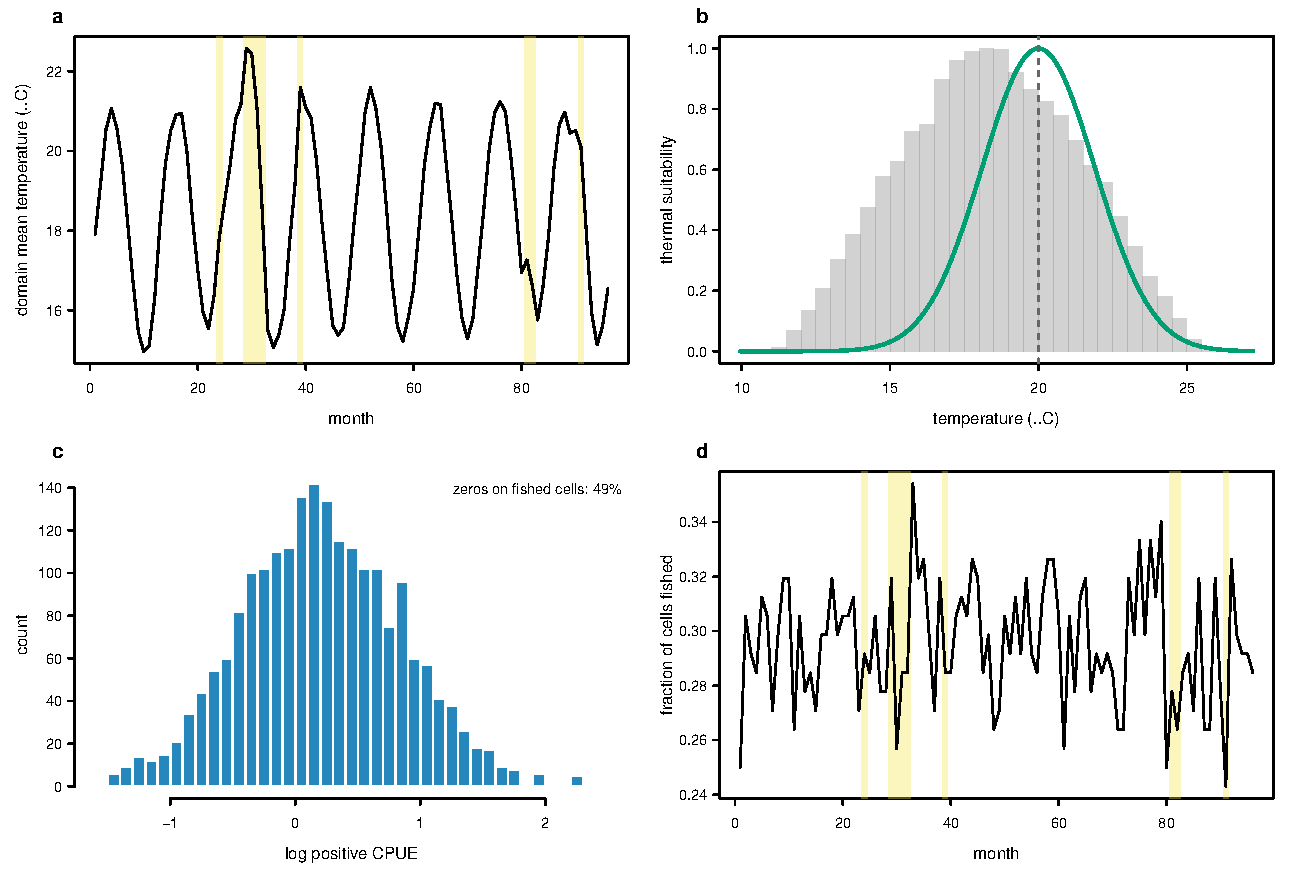
\includegraphics[width=0.9\linewidth]{fig2_data_distributions.pdf}
\caption{Simulated observations in a replicate with every mechanism active. (a) Mean temperature over the grid, with heatwave months shaded. (b) The thermal suitability curve, with the distribution of realised temperatures behind it. (c) Distribution of log positive CPUE, with the share of fished grid cells returning zero catch. (d) Share of grid cells fished in each month.}
\label{fig:S1}
\end{figure}

\begin{figure}[htbp]
\centering
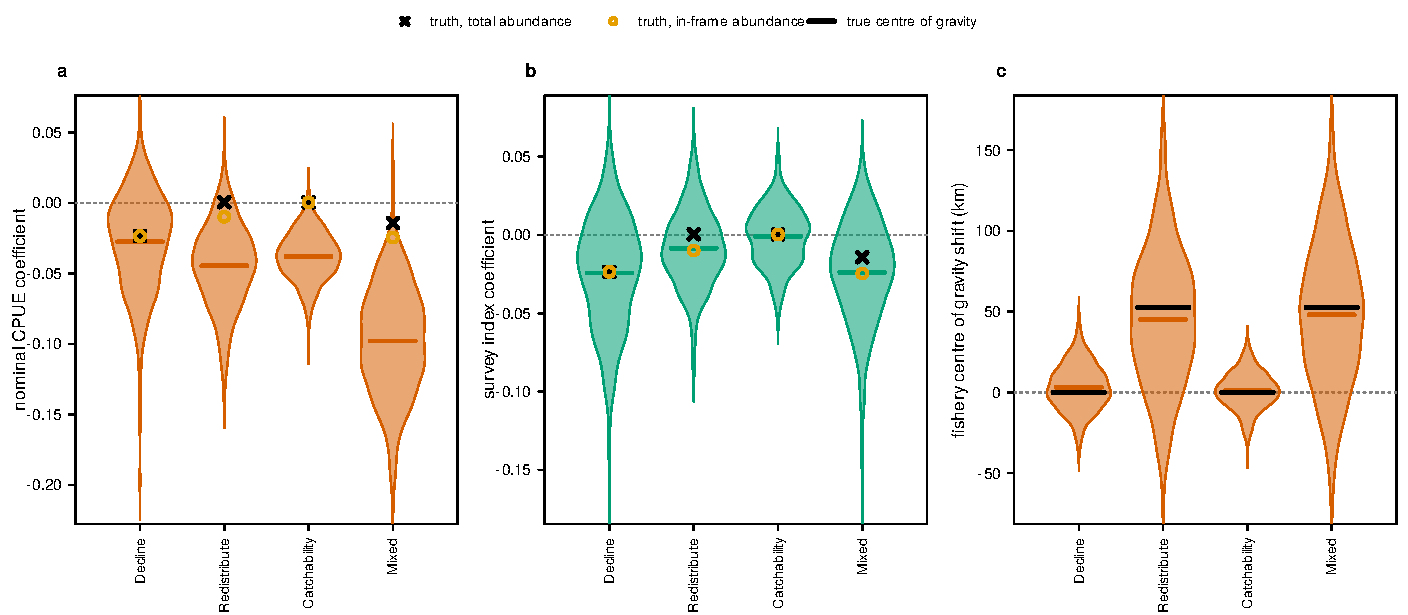
\includegraphics[width=\linewidth]{fig4_sampling_distributions.pdf}
\caption{Sampling distributions over 400 replicates for four scenarios with fleet contraction active (violins, with the replicate mean as a bar). (a) Nominal CPUE coefficient; (b) survey index coefficient; in both, the effect on total abundance is the black cross and the effect on in-frame abundance the orange circle. (c) Shift in the fishery's centre of gravity during events (km), with the true shift as the black bar.}
\label{fig:S2}
\end{figure}

\begin{figure}[htbp]
\centering
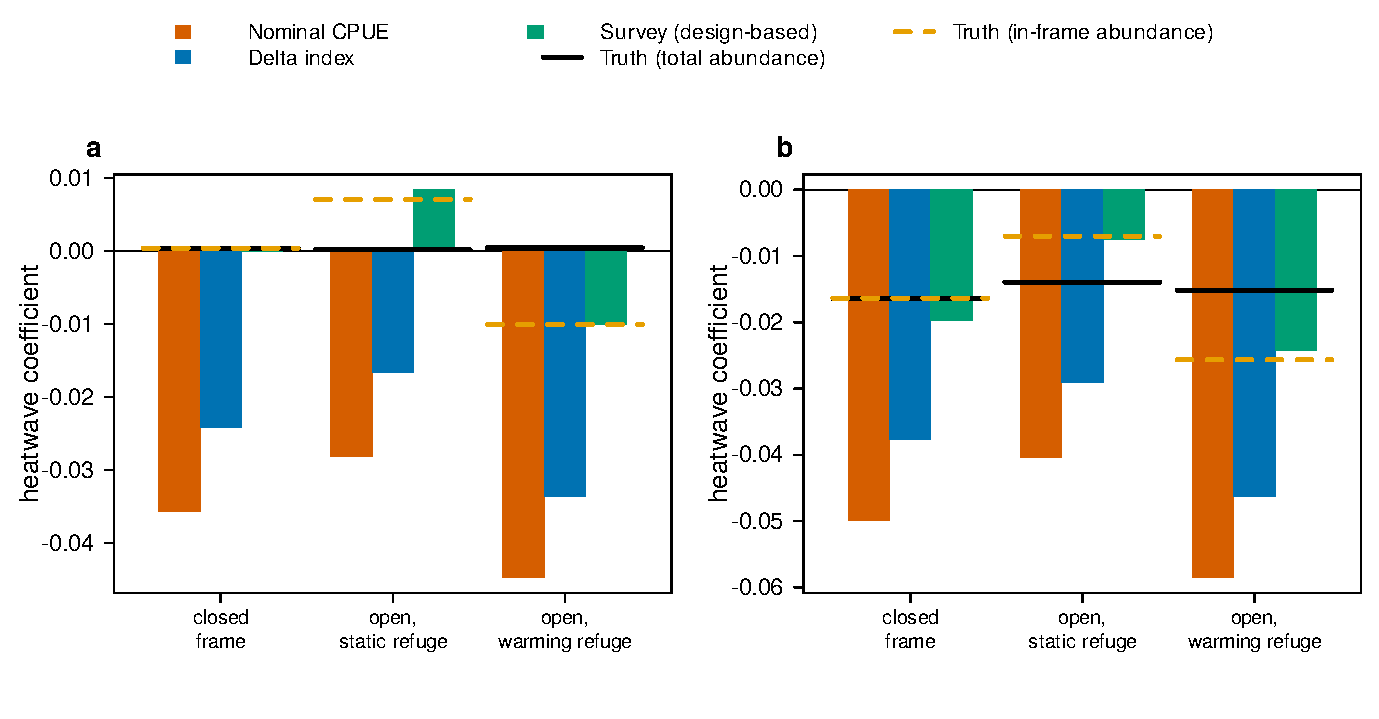
\includegraphics[width=\linewidth]{fig10_frame_geometry.pdf}
\caption{Frame geometry, with fleet contraction active (250 replicates per setting). (a) Redistribution only; (b) abundance decline and redistribution. Heatwave coefficients of the nominal, delta and survey indices against the effect on total abundance (black) and on in-frame abundance (orange dashed), for a closed frame, an open frame with a refuge of fixed suitability, and an open frame whose refuge warms with the frame (the default). The survey tracks in-frame abundance in every setting; which way in-frame abundance moves depends on whether the refuge warms.}
\label{fig:frame}
\end{figure}

\begin{figure}[htbp]
\centering
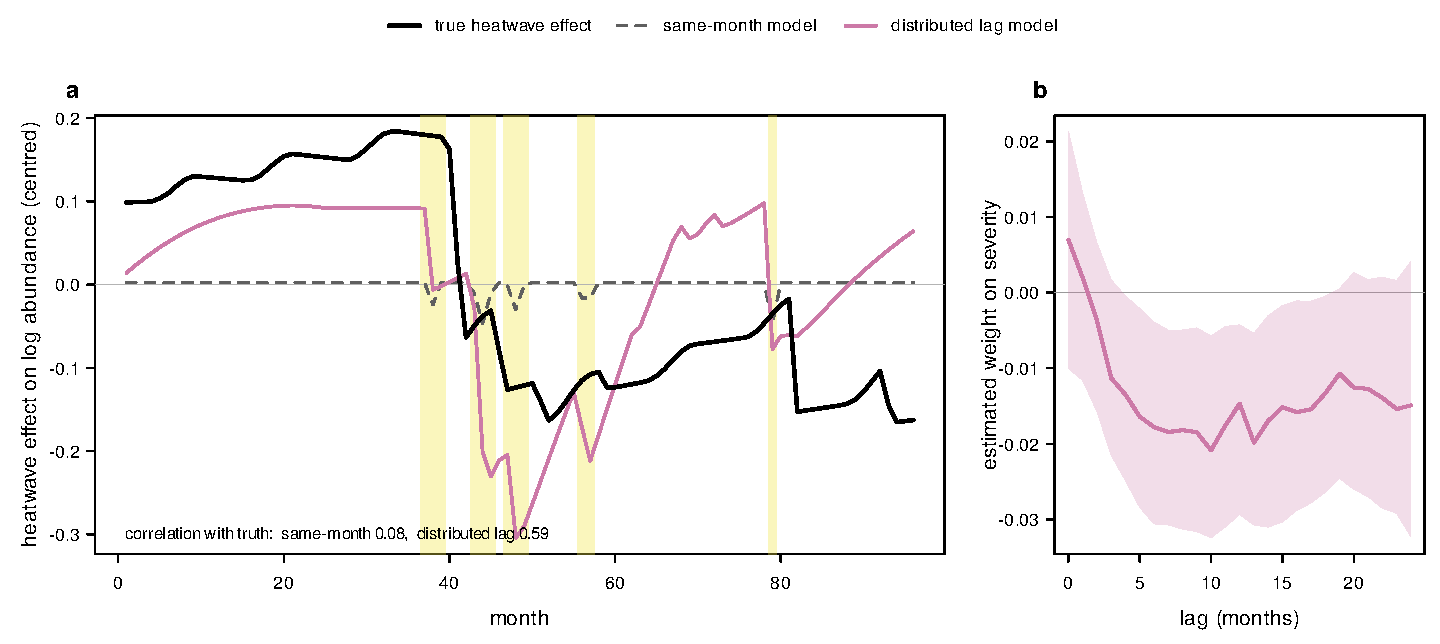
\includegraphics[width=\linewidth]{fig7_temporal.pdf}
\caption{Recovery of a lagged, cumulative decline from the observed survey index. (a) One replicate: the true heatwave effect on log abundance (black) and the fits of a same-month model (grey dashed) and a penalised distributed lag model (sky blue) to the detrended survey index, on a common centred scale, with heatwave months shaded and the correlation of each fit with the truth annotated. (b) Estimated distributed lag weights across 300 replicates (mean and interquartile band), with smoothing chosen by generalised cross-validation.}
\label{fig:temporal}
\end{figure}

\clearpage
%%BIBLIOGRAPHY%%

\end{document}
